% Blatt 2 — Lesen · Sprechen · Hören
% Kompilieren mit: lualatex interaktiv.tex
\documentclass[11pt,a4paper,DIV=12]{scrartcl}
% Gemeinsame Praeambel fuer alle Blaetter.
% Einbinden mit % Gemeinsame Praeambel fuer alle Blaetter.
% Einbinden mit % Gemeinsame Praeambel fuer alle Blaetter.
% Einbinden mit \input{../../stil.tex} — Pfad ist relativ zum Kompilierordner.
% Kompiliert wird mit lualatex (wegen luatexja).

\usepackage[ngerman]{babel}
\usepackage[haranoaji]{luatexja-preset}
\usepackage{luatexja-ruby}
\usepackage{booktabs}
\usepackage{array}
\usepackage{xcolor}
\usepackage[most]{tcolorbox}
\usepackage{enumitem}
\usepackage{microtype}
\usepackage{graphicx}
\usepackage{wrapfig}
\usepackage{multicol}
\usepackage{amssymb}
\usepackage{needspace}

% Gedankenstriche als LATEINISCHE Zeichen behandeln.
% luatexja haelt sie sonst fuer Japanisch — und weil japanische Zeichen
% keine Leerzeichen brauchen, frisst es den Zeilenumbruch danach:
% "Nomen —und wenn" statt "Nomen — und wenn".
\ltjdefcharrange{100}{"2013,"2014}
\ltjsetparameter{jacharrange={-100}}
\graphicspath{{../../bilder/}}

\definecolor{akzent}{HTML}{1F4E79}
\definecolor{implizit}{HTML}{1B7A43}
\definecolor{explizit}{HTML}{B3541E}
\definecolor{hell}{HTML}{F4F6F8}

\addtokomafont{disposition}{\color{akzent}}
\setkomafont{title}{\color{akzent}\bfseries}

\newcommand{\impl}{\textcolor{implizit}{\textbf{implizit}}}
\newcommand{\expl}{\textcolor{explizit}{\textbf{explizit}}}
\newcommand{\jterm}[2]{\ruby{#1}{#2}}

% Deutsche Anfuehrungszeichen: babel-Befehle statt Unicode.
% Sonst zwei Probleme: ASCII-" ist bei ngerman ein Umlaut-Shorthand
% ("o -> oe), und luatexja haelt Unicode-Quotes fuer Japanisch und
% setzt Abstand drumrum.
\newcommand{\zitat}[1]{\glqq #1\grqq{}}

% Schreiblinie fuer Antworten
\newcommand{\lin}[1][4cm]{\rule[-0.5em]{#1}{0.4pt}}

\newtcolorbox{merke}[1][]{
  enhanced, colback=hell, colframe=akzent,
  boxrule=0pt, leftrule=3pt, arc=0pt, outer arc=0pt,
  left=8pt, right=8pt, top=6pt, bottom=6pt,
  #1
}
 — Pfad ist relativ zum Kompilierordner.
% Kompiliert wird mit lualatex (wegen luatexja).

\usepackage[ngerman]{babel}
\usepackage[haranoaji]{luatexja-preset}
\usepackage{luatexja-ruby}
\usepackage{booktabs}
\usepackage{array}
\usepackage{xcolor}
\usepackage[most]{tcolorbox}
\usepackage{enumitem}
\usepackage{microtype}
\usepackage{graphicx}
\usepackage{wrapfig}
\usepackage{multicol}
\usepackage{amssymb}
\usepackage{needspace}

% Gedankenstriche als LATEINISCHE Zeichen behandeln.
% luatexja haelt sie sonst fuer Japanisch — und weil japanische Zeichen
% keine Leerzeichen brauchen, frisst es den Zeilenumbruch danach:
% "Nomen —und wenn" statt "Nomen — und wenn".
\ltjdefcharrange{100}{"2013,"2014}
\ltjsetparameter{jacharrange={-100}}
\graphicspath{{../../bilder/}}

\definecolor{akzent}{HTML}{1F4E79}
\definecolor{implizit}{HTML}{1B7A43}
\definecolor{explizit}{HTML}{B3541E}
\definecolor{hell}{HTML}{F4F6F8}

\addtokomafont{disposition}{\color{akzent}}
\setkomafont{title}{\color{akzent}\bfseries}

\newcommand{\impl}{\textcolor{implizit}{\textbf{implizit}}}
\newcommand{\expl}{\textcolor{explizit}{\textbf{explizit}}}
\newcommand{\jterm}[2]{\ruby{#1}{#2}}

% Deutsche Anfuehrungszeichen: babel-Befehle statt Unicode.
% Sonst zwei Probleme: ASCII-" ist bei ngerman ein Umlaut-Shorthand
% ("o -> oe), und luatexja haelt Unicode-Quotes fuer Japanisch und
% setzt Abstand drumrum.
\newcommand{\zitat}[1]{\glqq #1\grqq{}}

% Schreiblinie fuer Antworten
\newcommand{\lin}[1][4cm]{\rule[-0.5em]{#1}{0.4pt}}

\newtcolorbox{merke}[1][]{
  enhanced, colback=hell, colframe=akzent,
  boxrule=0pt, leftrule=3pt, arc=0pt, outer arc=0pt,
  left=8pt, right=8pt, top=6pt, bottom=6pt,
  #1
}
 — Pfad ist relativ zum Kompilierordner.
% Kompiliert wird mit lualatex (wegen luatexja).

\usepackage[ngerman]{babel}
\usepackage[haranoaji]{luatexja-preset}
\usepackage{luatexja-ruby}
\usepackage{booktabs}
\usepackage{array}
\usepackage{xcolor}
\usepackage[most]{tcolorbox}
\usepackage{enumitem}
\usepackage{microtype}
\usepackage{graphicx}
\usepackage{wrapfig}
\usepackage{multicol}
\usepackage{amssymb}
\usepackage{needspace}

% Gedankenstriche als LATEINISCHE Zeichen behandeln.
% luatexja haelt sie sonst fuer Japanisch — und weil japanische Zeichen
% keine Leerzeichen brauchen, frisst es den Zeilenumbruch danach:
% "Nomen —und wenn" statt "Nomen — und wenn".
\ltjdefcharrange{100}{"2013,"2014}
\ltjsetparameter{jacharrange={-100}}
\graphicspath{{../../bilder/}}

\definecolor{akzent}{HTML}{1F4E79}
\definecolor{implizit}{HTML}{1B7A43}
\definecolor{explizit}{HTML}{B3541E}
\definecolor{hell}{HTML}{F4F6F8}

\addtokomafont{disposition}{\color{akzent}}
\setkomafont{title}{\color{akzent}\bfseries}

\newcommand{\impl}{\textcolor{implizit}{\textbf{implizit}}}
\newcommand{\expl}{\textcolor{explizit}{\textbf{explizit}}}
\newcommand{\jterm}[2]{\ruby{#1}{#2}}

% Deutsche Anfuehrungszeichen: babel-Befehle statt Unicode.
% Sonst zwei Probleme: ASCII-" ist bei ngerman ein Umlaut-Shorthand
% ("o -> oe), und luatexja haelt Unicode-Quotes fuer Japanisch und
% setzt Abstand drumrum.
\newcommand{\zitat}[1]{\glqq #1\grqq{}}

% Schreiblinie fuer Antworten
\newcommand{\lin}[1][4cm]{\rule[-0.5em]{#1}{0.4pt}}

\newtcolorbox{merke}[1][]{
  enhanced, colback=hell, colframe=akzent,
  boxrule=0pt, leftrule=3pt, arc=0pt, outer arc=0pt,
  left=8pt, right=8pt, top=6pt, bottom=6pt,
  #1
}


\title{Blatt 2 — Lesen · Sprechen · Hören}
\subtitle{読む · 話す · 聞く}
\date{}
\author{}

\begin{document}
\maketitle
\vspace{-2.5em}

Alles nur Stoff aus Stunde 1 + 2, Vokabeln WaniKani Level 1–3.

Manche Nomen haben einen \textbf{ganzen Satz davor} (Relativsatz):
木を切る\textbf{父} = „der Vater, der Holz schneidet". Der Satz behält seine Partikel.

\section{Lesen （よむ）}

\begin{wrapfigure}{r}{3.2cm}
  \vspace{-1.6\baselineskip}
  
\includegraphics[width=3cm]{study_gogaku_woman_reading.png}
  \vspace{-1.6\baselineskip}
\end{wrapfigure}
Lies laut vor.

\begin{merke}
\begin{center}
\begin{tabular}{@{}l@{}}
大きい犬が入る。\\
犬は目が大きい。\\
犬を\jterm{引}{ひ}く子は小さい。\\
子が手を上げる。\\
手を上げた子が立つ。\\
木を\jterm{切}{き}る\jterm{父}{ちち}が入る。\\
父は大きい人。\\
犬が出る。\\
子は手を下げる。\\
\end{tabular}
\end{center}
\end{merke}

\textbf{Fragen} (antworte auf Japanisch):

\begin{enumerate}[itemsep=4pt]
\item 犬は大きい？
\item 犬は目が大きい？
\item 犬を引く子は大きい？
\item 手を上げた子は立つ？
\item \jterm{誰}{だれ}が木を切る？
\end{enumerate}

\section{Sprechen （はなす）}

\begin{wrapfigure}{r}{3.2cm}
  \vspace{-1.6\baselineskip}
  
\includegraphics[width=3cm]{study_gogaku_woman_speaking.png}
  \vspace{-1.6\baselineskip}
\end{wrapfigure}
Sprich den Dialog — erst du B, dann tauschen wir.

\begin{center}
\begin{tabular}{@{}ll@{}}
A：これは犬？ & \\
B：ええ、犬。大きい犬。 & \\
A：犬は目が大きい？ & \\
B：ええ、大きい。 & \\
A：犬を引く子は大きい？ & \\
B：小さい。犬を引く子は小さい。 & \\
A：木を切る人は父？ & \\
B：ええ、父。 & \\
A：犬が出る？ & \\
B：ええ、出る。 & \\
\end{tabular}
\end{center}

Danach frei: Ich zeig auf etwas oder frag, du antwortest — Prädikat wiederholen oder
korrigieren.

\section{Hören （きく）}

\begin{wrapfigure}{r}{3.2cm}
  \vspace{-1.6\baselineskip}
  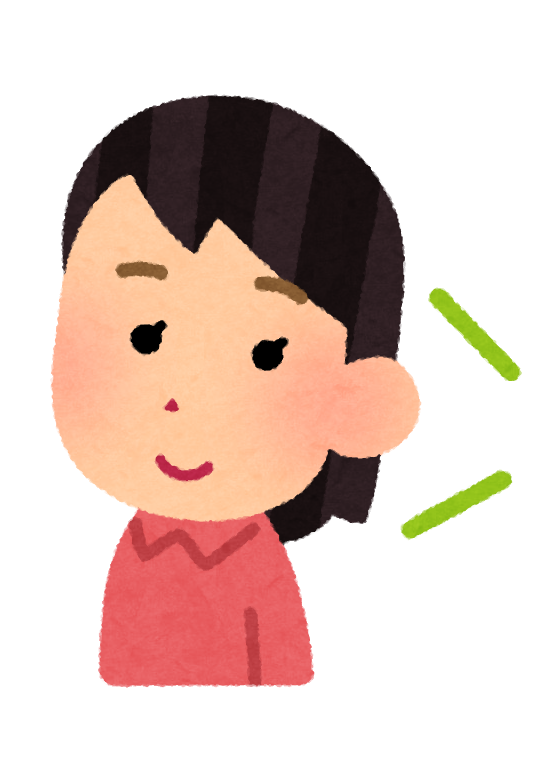
\includegraphics[width=3cm]{study_gogaku_woman_listning.png}
  \vspace{-1.6\baselineskip}
\end{wrapfigure}
Du hörst nur zu — ich lese vor. Beantworte danach die Fragen.

\textbf{Fragen für dich:}

\begin{enumerate}[itemsep=4pt]
\item \jterm{牛}{うし}は大きい？
\item 牛は目が大きい？
\item 牛を引く人は大きい？
\item 牛が出る？
\item \jterm{誰}{だれ}が木を切る？
\end{enumerate}

\bigskip
\rule{\linewidth}{0.4pt}

\textbf{Nur für den Lehrer — Hörtext} (vorlesen, nicht zeigen):

\begin{merke}
\begin{tabular}{@{}l@{}}
小さい牛が立つ。\\
牛は目が小さい。\\
牛を\jterm{引}{ひ}く人は大きい。\\
手を上げた子が入る。\\
木を\jterm{切}{き}る\jterm{父}{ちち}が立つ。\\
牛が出る。\\
子は手を下げる。\\
\end{tabular}
\end{merke}

\end{document}
